\subsubsection{Pivoting by rows (partial pivoting)}

\begin{flushleft}
    \textcolor{Green3}{\faIcon{question-circle} \textbf{Purpose and Goal}}
\end{flushleft}
\begin{itemize}
    \item \textbf{Prevent Division by Zero}. Ensure that the pivot element is non-zero.
    \item \textbf{Improve Numerical Stability}. Minimize rounding errors and improve the accuracy of the solution.
\end{itemize}
The \textbf{goal} is to ensure that the pivot element is the largest possible value in the current column.

\highspace
\begin{flushleft}
    \textcolor{Green3}{\faIcon{tools} \textbf{Algorithm}}
\end{flushleft}
For each column $k$ (from the first to the last):
\begin{enumerate}
    \item \important{Identify the Pivot Element}. \textbf{Find the row} $i$ (where $i > k$) \textbf{with the largest absolute value in the pivot column}.
    
    This ensures that the selected pivot element $a_{kk}$ is the largest possible, reducing the potential for numerical instability. From a mathematical point of view:
    \begin{equation*}
        \overline{i} \: : \: \left|
            a_{\overline{r}k}^{\left(k\right)}
        \right| = \underset{
            i > k
        }{\max}
        \left|
            a_{ik}^{\left(k\right)}
        \right|
    \end{equation*}


    \item \important{Swap Rows}. Swap row $k$ with row $i$ to move the largest pivot element to the diagonal position ($a_{kk}$). This is achieved by pre-multiplying the matrix $A$ by a permutation matrix $P$, which swaps the rows in the identity matrix $I$.

    \item \important{Update the Matrix and Vector}. Perform the standard row operations to eliminate the elements below the pivot element, resulting in an upper triangular matrix. Update the constants vector accordingly.
\end{enumerate}
\begin{figure}[!htp]
    \centering
    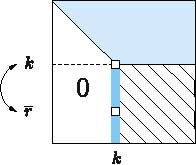
\includegraphics[width=.4\textwidth]{img/pivoting-by-rows-1.pdf}
\end{figure}